% ==============================================================================
\chapter{Simulation and reconstruction software frameworks}
\label{ch:Software}
%==============================================================================    

Simulation tools have a crucial role in the development and also
understanding of the performance of semiconductor devices. The
simulations are validated with the data and used to predict the
performance of small-pitch pixels for which data is not yet available.

This chapter describes the simulation tools used to understand the
performance of Timepix3 devices. The reconstruction software, used for
both data and simulation, is also presented.

%% --------------------------------------------- %%
\section{\textsc{Geant4}}\label{sec:Silicon_Geant4}

\textsc{Geant4}~\cite{Agostinelli:2002hh}, as an object-oriented
simulation toolkit implemented in the C++ programming language, is
widely used in high energy, nuclear and accelerator physics, medical
and space sciences. As modern particle physics is going towards
large-scale detectors, more accurate simulations are needed in order
to understand the complex situations. \textsc{Geant4} provides
software components which can be used to study basic phenomena,
geometries and full-scale detector simulations for
experiments. \textsc{Geant4} simulations take into account parameters
such as: the geometry of the system, the materials involved, the
generation of primary particles, the tracking of particles through
materials and external electromagnetic fields, the physics processes
involved in the possible interaction of the particles with the
materials they are passing through, the response of sensitive
components. The simulations of the interaction between the particles
and materials are mostly validated with data. In this thesis, all the
studies using \textsc{Geant4} are done with version 10.1.2.

\textsc{Geant4} provides physics models for different type of
interactions called \textit{physics lists}. The \textit{emstandard}
physics lists provide the electromagnetic interactions of photons and
charged particles with matter and is suited for the simulation of
ionisation, bremsstrahlung, gamma conversion and other electromagnetic
interactions of particles with energies from $1\,\kev$ up to
$10\,\pev$~\cite{Apostolakis2009859}. This physics list is commonly
used for the simulation of the energy loss in pixel detectors.

\textsc{Geant4} provides as well the Photo-Absorption Ionisation (PAI)
model~\cite{Apostolakis:2000yu} for the precise simulation of
ionisation energy loss by relativistic charged particles in very thin
absorbers. Since in very thin sensors the Landau model is not suitable
(see \cref{sec:landau}), the PAI model is based on the
photo-absorption cross-section tables obtained by experimental
data. In practice several classes are used to calculate the integral
ionisation cross-section, the mean number of ionising collisions as
well as the mean ionisation energy loss for the selected material and
the given Lorentz factor.



\cref{fig:BichselVSG4} compares the energy loss due to ionisation in
$50\,\micron$ and $450\,\micron$ thick silicon sensors for different
\textsc{Geant4} physics lists and the Bichsel parametrisation
(see~\cref{sec:bichsel}). For the $50\,\micron$ thick sensor, the
\textit{emstandard\_opt3} physics list gives a reasonable value for
the most probable value ($\Delta_p$) but the width ($w$) of the
distribution is more narrow than the Bichsel distribution. The PAI
model shows a very good agreement with the Bichsel model. For the
thick sensor of $450\,\micron$, both PAI and emstandard\_opt3 physics
lists show similar distributions as the Bichsel model.

The energy deposition given by the PAI model is very close to the one
calculated by Bichsel especially for the fluctuations around the most
probable value and for very thin sensors. For this reason, the PAI
model is chosen to be used later for the simulations even though it
requires more computation power.
 
\begin{figure}[htbp] \centering
  \begin{subfigure}[b]{0.45\textwidth}
    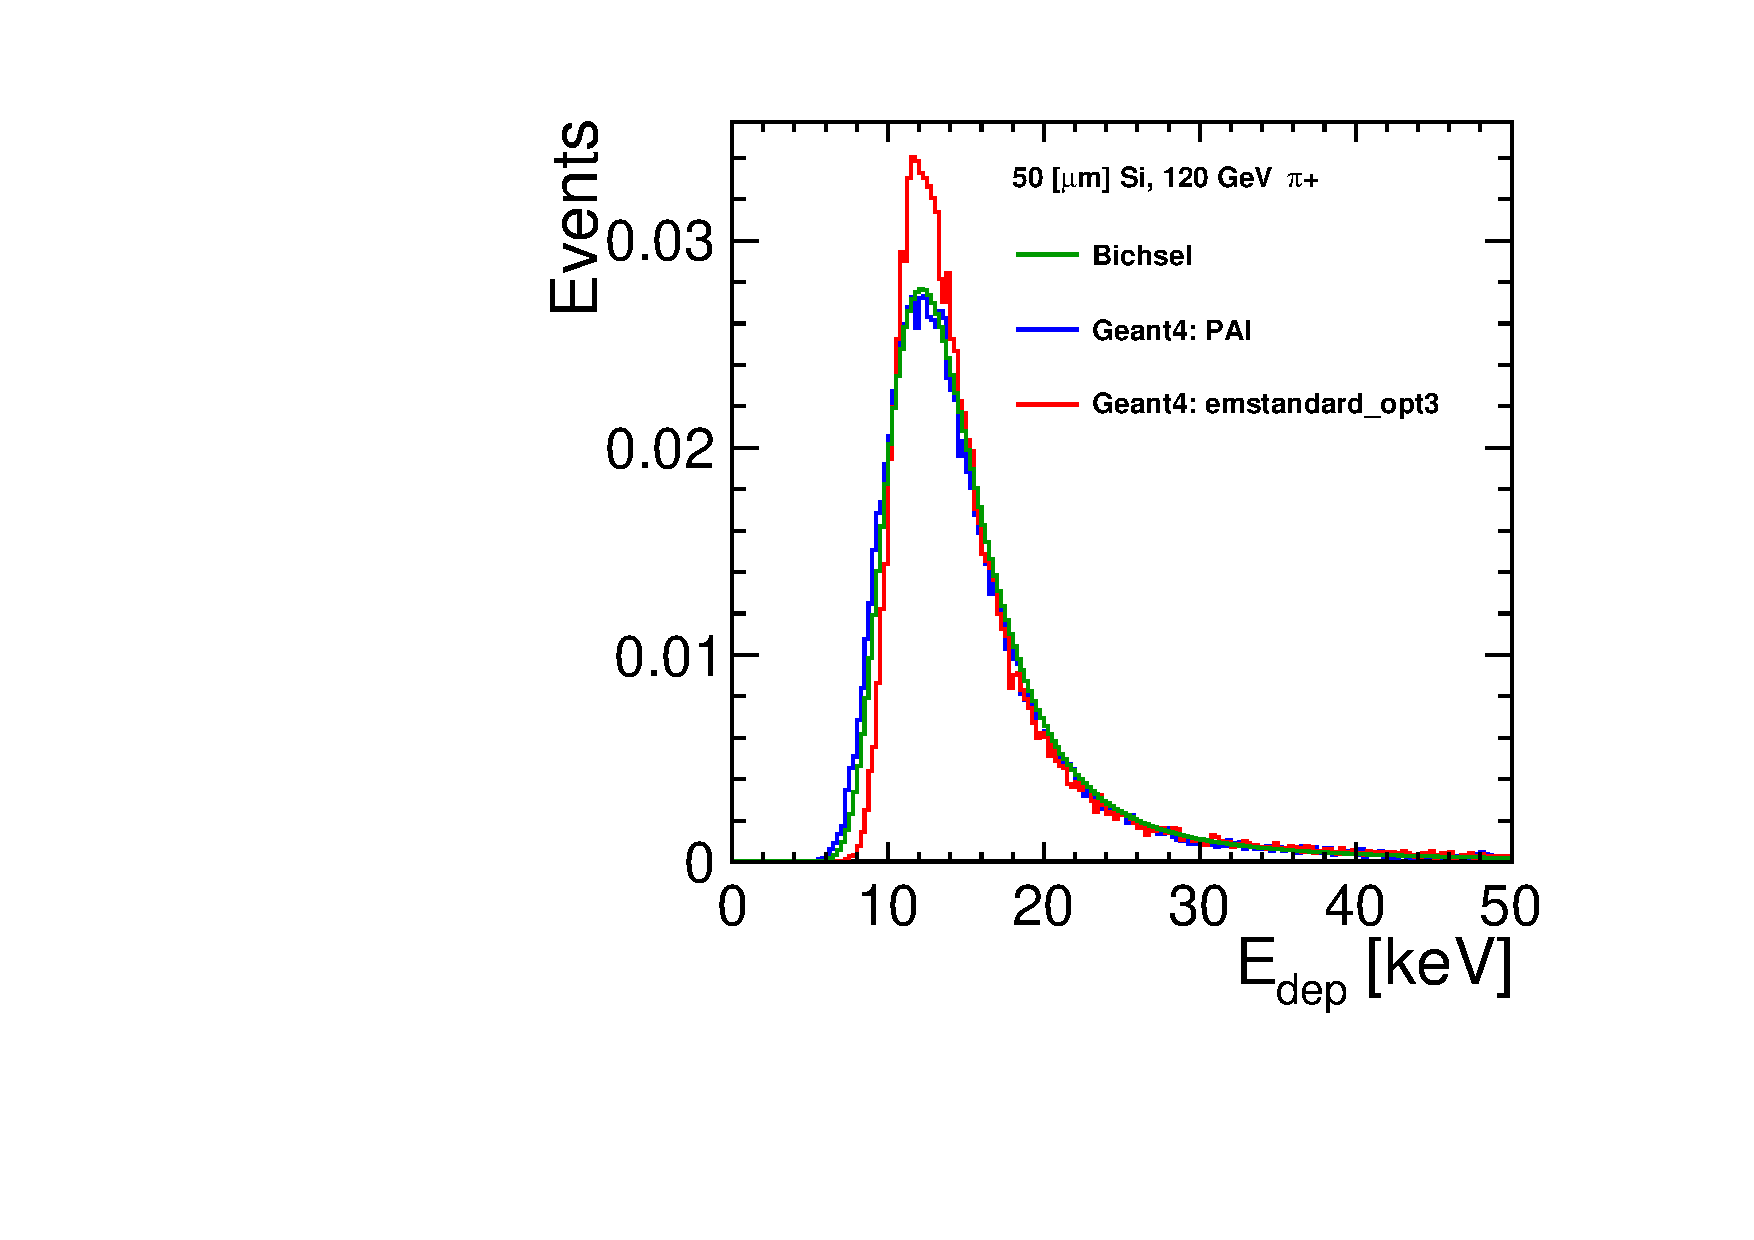
\includegraphics[width=\textwidth]{figures/ChargeSharing/50um_bichsel_physicsLists.pdf}
    \caption{}
  \end{subfigure} \hfill
  \begin{subfigure}[b]{0.45\textwidth}
    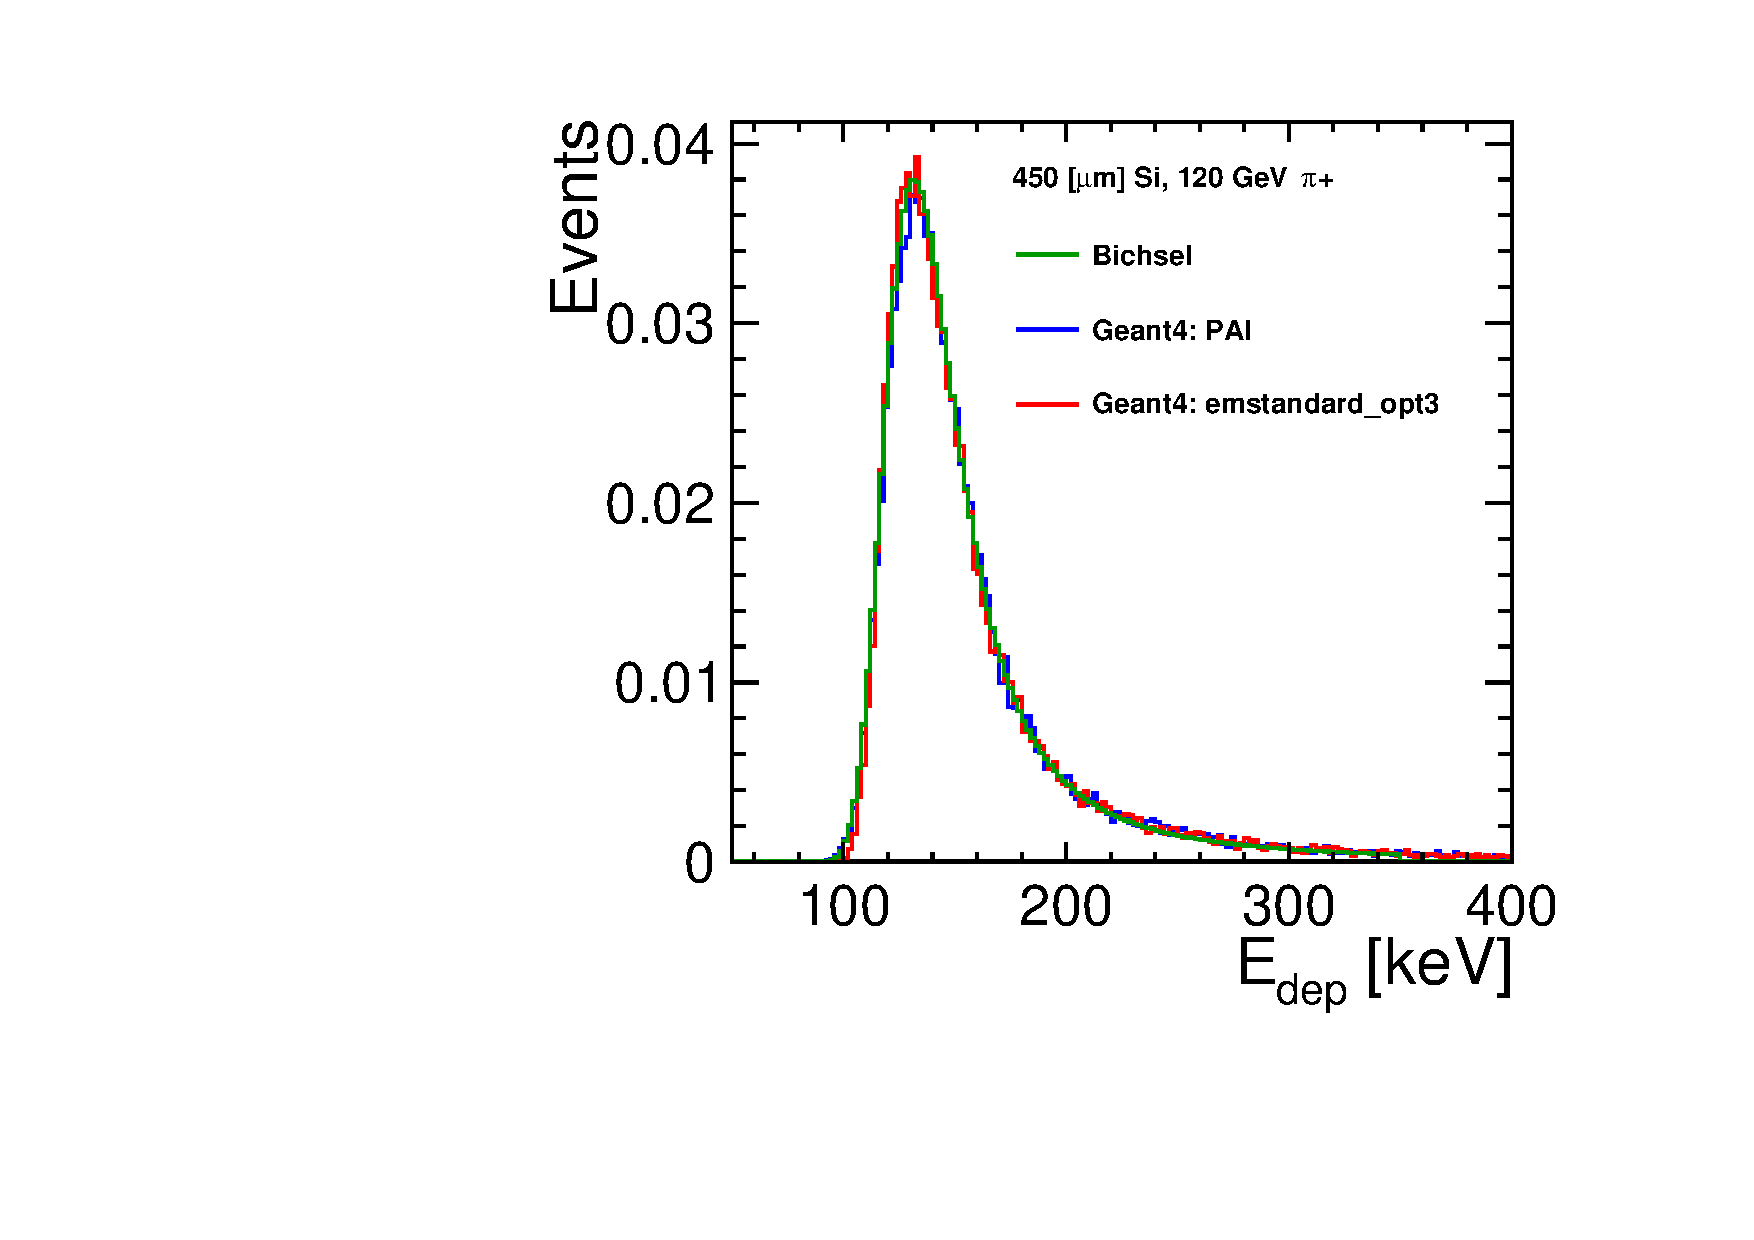
\includegraphics[width=\textwidth]{figures/ChargeSharing/450um_bichsel_physicsLists.pdf}
    \caption{}
  \end{subfigure}
  \caption{Energy-loss distribution in (a) $50\,\micron$ and (b)
    $450\,\micron$ thick silicon sensors by $120\,\gev$ $\pi^{+}$
    comparing the Bichsel model and \textsc{Geant4} using the PAI and
    the emstandard\_opt3 physics lists.}
  \label{fig:BichselVSG4}
\end{figure}

%% --------------------------------------------- %%
\section{AllPix simulation framework}
\label{sec:AllPix}

AllPix~\cite{Benoit:1474878,allpix,allpixTwiki} is a
\textsc{Geant4}-based simulation software framework. It is written in
C/C++ and provides a flexible interface to define a pixel detector
geometry to simulate pixelated sensors and readout chips. It is widely
used for the simulation of pixel detectors in different high energy
physics experiments. It allows for defining an experimental setup with
its surrounding environment as realistic as possible, such as the
components of a test beam setup. It also allows for the simulation of
more complexe geometries such as a full vertex detector.

\textsc{Geant4} provides the simulation of particles through the
matter: it calculates the position of the hits (the true Monte Carlo
position) considering multiple scattering and the energy deposition in
the sensitive volumes (sensors). The software user defines the
semiconductor physics and readout chip properties in a digitiser as
described below.

\cref{fig:TPX3TelescopeAllpix} shows an example of the simulation for
the Timepix3 telescope (described in \cref{ch:Telescope}) in AllPix
with the device under test (DUT) in the middle of the tilted telescope
planes.

\begin{figure}[htbp]
  \centering
  \begin{tikzpicture}
    \node[anchor=south west,inner sep=0] (image) at
    (0,0){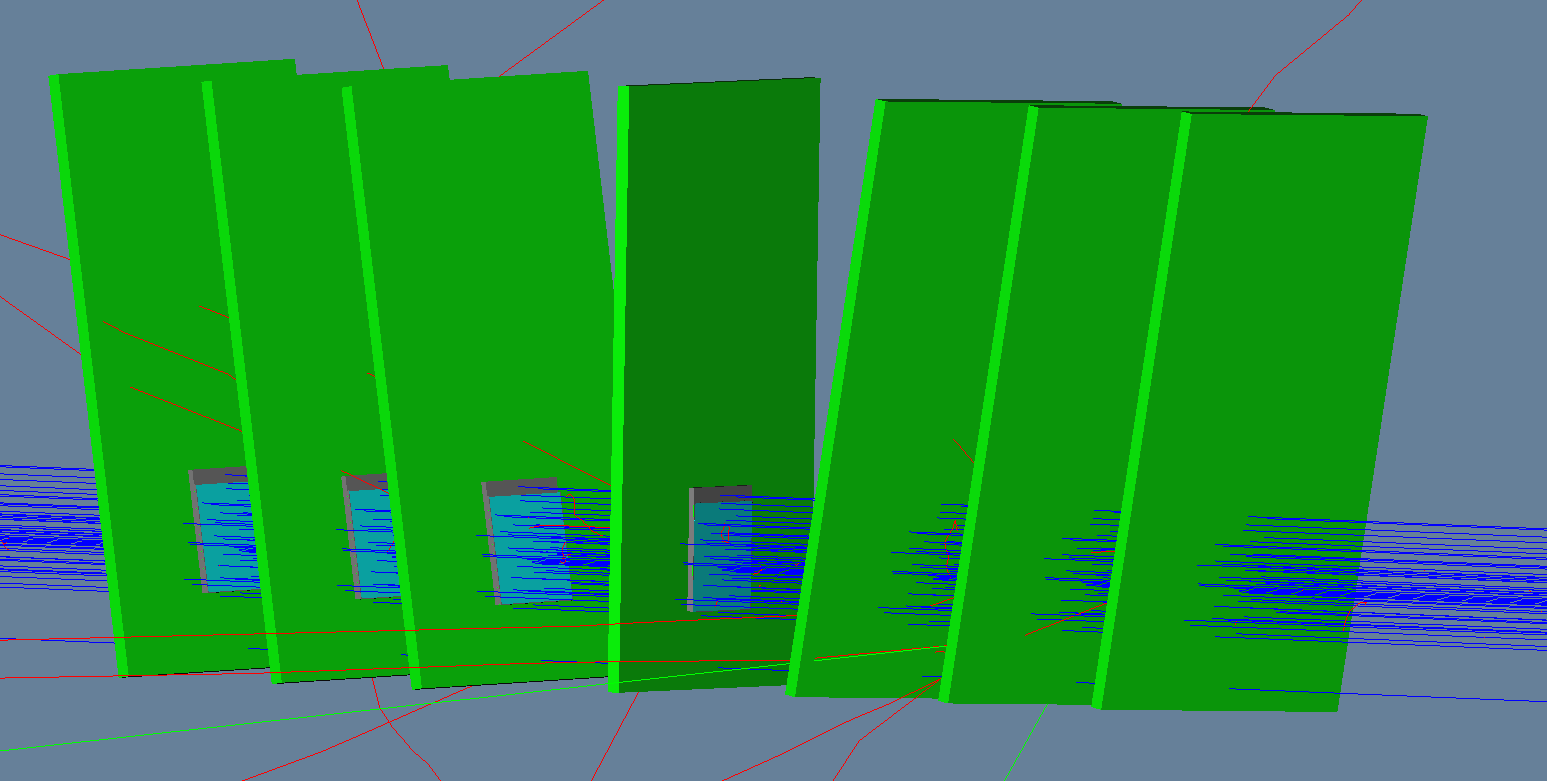
\includegraphics[width=0.8\textwidth]{figures/ActiveEdge/Allpix_telescope_withParticles.png}};
    \begin{scope}[x={(image.south east)},y={(image.north west)}]
      \node[above, color=white] at (0.53, 0.65) {\textbf{DUT}};
    \end{scope}
  \end{tikzpicture}
  \caption{Simulation of the Timepix3 telescope in AllPix with the six
    tilted telescope planes and the device under test (DUT) in the
    center as well as particle tracks from the beam entering the
    telescope from the right.}
  \label{fig:TPX3TelescopeAllpix}
\end{figure}

%% --------------------------------------------- %%
\subsection{Coordinate system}

The convention used for the pixel detectors (in AllPix and also in the
reconstruction software as described in \cref{sec:recoSoft}) for a
Timepix3-like matrix of $256\times256$ pixels is shown in
\cref{fig:coordinateSystem}. The pixel coordinates (column, row) are
shown in black and the local coordinates (x, y) in millimeters of the
center of the pixels in the corners of the matrix are shown in
blue. In this convention we are looking from the sensor side with the
periphery at the bottom.

\begin{figure}[htbp]
  \centering
  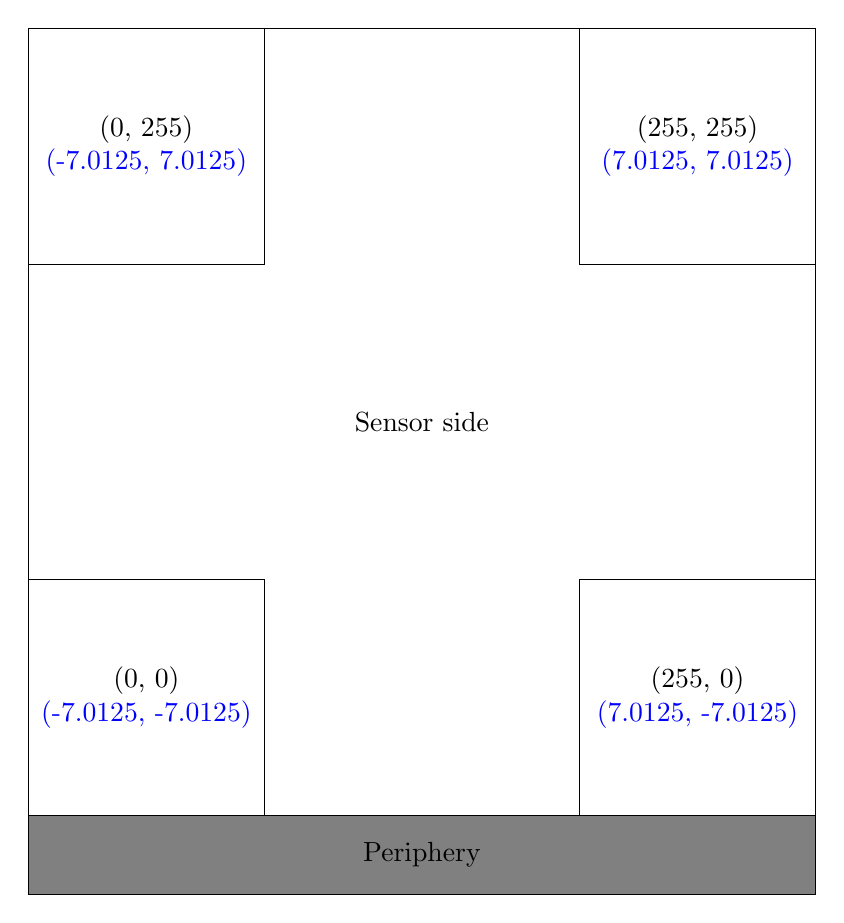
\begin{tikzpicture}
    \begin{scope} 

      \draw (0, 0) rectangle (10, 10) node[pos=.5] {Sensor side};
      \draw[fill=gray] (0, -1) rectangle (10, 0) node[pos=.5]
      {Periphery};

      \draw (0, 10) rectangle (3, 7) node[align=center, pos=.5] {(0, 255) \\ \textcolor{blue}{(-7.0125, 7.0125)}};
      \draw (7, 10) rectangle (10, 7) node[align=center, pos=.5] {(255,
        255) \\ \textcolor{blue}{(7.0125, 7.0125)}};
      
      \draw (0, 0) rectangle (3, 3) node[align=center, pos=.5]{(0, 0) \\ \textcolor{blue}{(-7.0125, -7.0125)}};
      \draw (7, 0) rectangle (10, 3) node[align=center, pos=.5] {(255, 0) \\ \textcolor{blue}{(7.0125, -7.0125)}};
    \end{scope}  
  \end{tikzpicture}
  \caption{The coordinates system for a matrix of $256\times256$
    pixels. The pixel coordinates (column, row) are shown in black and
    the local coordinates (x, y) in millimeters of the center of the
    pixels in the corners of the matrix are shown in blue. In this
    convention, we are looking from the sensor side with the periphery
    at the bottom.}
  \label{fig:coordinateSystem}
\end{figure}
%% --------------------------------------------- %%
\subsection{Geometry of the pixel detector}

In AllPix, the pixel detector geometry can be defined by the pitch
size, the thickness of the sensor and the readout chip for a hybrid
configuration, the PCB properties, the mechanical support and other
geometry properties related to an assembly. These parameters are
usually defined in an XML file. Each detector is identified by a
unique ID number. This facilitates the running of the simulation with
different parameters by only changing the XML file without the need of
re-compiling the code. It is also possible to define the parameters of
the digitiser in this XML file.
%% --------------------------------------------- %%
\subsection{Geometry of the simulation scenario}

The simulation scenario is defined in a macro file. The position of
the detectors in space is specified by the coordinates (x, y, z) and
the rotations around the x, y and z axes of the centre of the
detectors. The physics list used by \textsc{Geant4} is specified. The
General Particle Source (GPS), which is the \textsc{Geant4} toolkit
for the generation of high-energy particles, is also described in the
macro file. The particle type, the beam energy, position and
distributions are customisable. The simulation is done based on
frames. The frame can be related to the integration time of the
detectors during which the shutter is open and all the particles are
detected in this specific lapse of time. For a Timepix3-like detector
which is operated based on a data-driven readout (see
\cref{sec:TimepixReadout}), the frame length is not fully defined. For
the simulation of such a readout, the beam profile is defined in such
a way that pile-ups are avoided and a pixel is hit by particles only
once during one simulation frame. During test beams, the particle rate
is also adjusted to avoid pile-ups. Since we are mostly interested in
the physics of the detector and not testing the timing capabilities of
the readout system, this definition of a frame is plausible.

Visualisation parameters are also given in the macro. Open
Inventor~\cite{OpenInventor} can be, for example, used to visualise
the simulation scenario and also the particle tracks in the detectors.

%% --------------------------------------------- %%
\subsection{Digitisation}
\label{sec:allpix_digitisation}

For each simulation step (\texttt{G4Step}) through the matter,
\textsc{Geant4} provides the energy deposited in the sensitive
material. The step length can be customised and for thin sensors
simulations, a step of $2\,\micron$ provides a good precision for the
calculations. 

The semiconductor physics in a silicon detector is defined in the
digitiser. The drift and diffusion are performed at each step to
simulate the electron-hole pair movement in the electric field. The
simplified model as described in \cref{sec:reversedBiasedPNjunction}
is used for the simulation of silicon physics. In practice at each
\texttt{G4Step}, where the energy deposition is given by
\textsc{Geant4}, the amount of the charges drifting towards the
readout electrode is known. These charges diffuse due to the random
thermal motion in the crystal lattice and do not exactly follow the
electric field lines. The spread of the arrival position of a charge
generated at a given Step\textsubscript{z} is described as a Gaussian
distribution with standard deviation as given in
\cref{eq:sigmaDiffusion}. \cref{fig:digitisation} schematically
illustrates the digitisation in a sensor in one direction. Each
\textsc{Geant4} step is shown in a circle. In 2D, at each step, the
contribution of the diffusion is calculated in the hit pixel and its
neighbouring pixels using:

\begin{equation}
Q(z)=q_i(z) \cdot {1\over{\sqrt{2\,\pi}\sigma(z)}} \int_{x_{1}}^{x_{2}} e^{-({{x-x_{hit}}\over{\sqrt{2}\,\sigma(z)}})^2} dx \cdot {1\over{\sqrt{2\,\pi}\sigma(z)}} \int_{y_{1}}^{y_{2}} e^{-({{y-y_{hit}}\over{\sqrt{2}\,\sigma(z)}})^2} dy 
\end{equation}

where $q_i(z)$ is the energy deposited at step i at the depth $z$,
$\sigma(z)$ the diffusion standard deviation at $z$, $x_{hit}$ and
$y_{hit}$ is the coordinates where the track hits a pixel, $x_1$ and
$x_2$ the x-coordinates and $y_1$ and $y_2$ the y-coordinates of the
pixel where the contribution of the charge is being calculated.

For each pixel, all contributions sum up and the total charge
deposited in a pixel is calculated.

\begin{figure}[htbp]
  \centering
  \begin{tikzpicture}[node distance = 2.5cm, auto]
    \begin{scope}[x={(image.south east)},y={(image.north west)}]
      
      \draw[thick] (0.2, 0.6) -- (0.8, 0.6);
      \draw[thick] (0.2, 0.2) -- (0.8, 0.2);

      \draw[thick] (0.2, 0.2) -- (0.2, 0.6);
      \draw[thick] (0.8, 0.2) -- (0.8, 0.6);  

      \draw[thick] (0.4, 0.2) -- (0.4, 0.6);  
      \draw[thick] (0.6, 0.2) -- (0.6, 0.6);  

      \draw[green, thick] (0.45, 0.2) circle (0.5mm);
      \node[right, color=green] at (0.45, 0.22) {Step 1};
      \draw[green, thick] (0.45, 0.2) -- (0.36, 0.6);  
      \draw[green, thick] (0.45, 0.2) -- (0.54, 0.6);
      \draw[green, thick, <->] (0.36, 0.62) -- (0.54, 0.62);
      \node[above, color=green] at (0.36, 0.62) {$\sigma(z1)$};

      \draw[red, thick] (0.473, 0.3) circle (0.5mm);
      \node[right, color=red] at (0.473, 0.32) {Step 2};
      \draw[red, thick] (0.473, 0.3) -- (0.403, 0.6);
      \draw[red, thick] (0.473, 0.3) -- (0.543, 0.6);
      \draw[red, thick, <->] (0.403, 0.64) -- (0.543, 0.64);
      \node[above, color=red] at (0.403, 0.64) {$\sigma_{2}$};

      \draw[cyan, thick] (0.5, 0.4) circle (0.5mm);
      \node[right, color=cyan] at (0.5, 0.42) {Step 3};
      \draw[cyan, thick] (0.5, 0.4) -- (0.45, 0.6);
      \draw[cyan, thick] (0.5, 0.4) -- (0.55, 0.6);
      \draw[cyan, thick, <->] (0.45, 0.66) -- (0.55, 0.66);
      \node[above, color=cyan] at (0.45, 0.66) {$\sigma_{3}$};

      \draw[purple, thick] (0.525, 0.5) circle (0.5mm);
      \node[right, color=purple] at (0.525, 0.52) {Step 4};
      \draw[purple, thick] (0.525, 0.5) -- (0.495, 0.6);
      \draw[purple, thick] (0.525, 0.5) -- (0.555, 0.6);
      \draw[purple, thick, <->] (0.495, 0.68) -- (0.555, 0.68);
      \node[above, color=purple] at (0.495, 0.68) {$\sigma_{4}$};

      \draw[blue, thick, ->] (0.4, 0.0) -- (0.6, 0.8);  
      \node[above, color=blue] at (0.6, 0.8) {MIP};
      \draw[black, thick, ->] (0.1, 0.2) -- (0.1, 0.6);  
      \node[left, color=black] at (0.1, 0.4) {E\textsubscript{field}};

      \draw[black, thick, ->] (0.9, 0.7) -- (0.9, 0.1);  
      \node[below, color=black] at (0.9, 0.1) {z};
      \draw[-] (0.89, 0.6) -- (0.91, 0.6) node[right] {0};

      \node[below, color=black] at (0.3, 0.15) {Pixel 1};
      \node[below, color=black] at (0.5, 0.15) {Pixel 2};
      \node[below, color=black] at (0.7, 0.15) {Pixel 3};

      %% \node at (4.5,4) 
      %% {some text spanning three lines with automatic line breaks};

      % \draw[help lines,xstep=.1,ystep=.1] (0, 0) grid (1,1);
      % \foreach \x in {0,1,...,9} { \node [anchor=north] at (\x/10,0) {0.\x}; }
      % \foreach \y in {0,1,...,9} { \node [anchor=east] at (0,\y/10) {0.\y}; }
    \end{scope}
  \end{tikzpicture}
  \caption{Illustration of the digitisation in a sensor. Each
    \textsc{Geant4} step (\texttt{G4Step}) is shown with a circle. The
    contribution of the diffusion ($\sigma_1$, $\sigma_2$, $\sigma_3$
    and $\sigma_4$) in the hit and its neighbouring pixels is
    calculated.}
  \label{fig:digitisation}
\end{figure}

The digitiser also defines the parameters of the readout chip. The
electronic noise (Gaussian distribution as described in
\cref{sec:noise}) is added. The readout threshold is applied to
eliminate the pixels where the charge deposition is less than the
threshold. The hit energy is converted to the digital value TOT
(time-over-threshold) using the readout calibrations (see
\cref{sec:EnergyCalibration}).


%% --------------------------------------------- %%
%% --------------------------------------------- %%
\section{TCAD simulations}
\label{sec:TCAD}
Technology Computer-Aided Design (TCAD) as a simulation tool is used
to optimise and develop semiconductor processing technologies as well
as the device operation~\cite{synopsysTCAD}. TCAD uses a finite
element method to numerically solve the physical partial differential
equations in semiconductors, such as the continuity and diffusion
equations. This allows for the modeling of the structural properties
and the electrical behaviour of semiconductor devices.

The TCAD simulations are performed in different steps. First, the
sensor geometry is defined in a 2D or a 3D configuration. The doping
profiles for the specific regions of the simulation are defined. In
this step, the wafer processing is imitated as it is done in a
foundry. The silicon bulk is doped to obtain the desired
resistivity. The pixel implants are deposited to form
pn-junctions. The aluminum contacts are placed to apply the high
voltage on the backside of the sensor and the ground on the
pixels. The simulation mesh is then described. The mesh divides the
surfaces and volumes into small triangles. The simulation is solved
numerically on this grid by respecting the boundary conditions and
continuity equations between the mesh points. The number of the mesh
points defines the accuracy and therefore the computation time for
solving the equations. An optimised definition of the mesh is crucial
for obtaining the solutions. Too coarse meshes may result in a poor
accuracy of the solutions or even the calculations might not
converge. For this reason, fine mesh points are described in regions
with high gradients in the doping profiles and close to the pixel
implants. Coarser mesh points are defined for the bulk of the sensor
where the doping concentration is almost constant.

The stationary solution at a certain bias voltage is obtained after
defining the geometry, the doping profiles and the mesh points. The
voltage on the backside contact is ramped up in small steps. The
electric field within the sensor is calculated and the depletion
volume is delimited.

Finally, a transient simulation can also be performed after a particle
hit in the sensor. Charge carriers are generated in the sensor by the
passing of ionising particles. The charge carriers are propagated for
a given time period. During their drifts towards the readout
electrodes, an induced current is also generated in the contacts. The
charge signal in the readout electrodes is integrated over the
integration time and the signal to get the signal the readout chip
would obtain.

For this study Synopsys TCAD version I-2013.12 is used to simulate the
movement of charge carriers in silicon and the coupling to the readout
as described in \cref{sec:RamoTheorem}. Also it is used to simulate
active-edge devices and compare with the measurements in
\cref{ch:ActiveEdgeSensors}.
%% --------------------------------------------- %%

%% --------------------------------------------- %%
\section{Reconstruction and analysis software frameworks}
\label{sec:recoSoft}

The offline reconstruction of the test beam data is done using two
software frameworks. The EUTelescope software
package~\cite{Rubinskiy,EutelescopeWebsite} is used to reconstruct the
tracks from the telescope and extrapolate their positions on the
DUT. For the analysis of the DUT data, the python-based software
pyEudetAnalysis is used~\cite{pyeudet}.

\subsection{EUTelescope}
\label{sec:EUTelescope}
The EUTelescope software is based on the ILCSoft
framework~\cite{Aplin:2009zz}. The latter provides the basic building
blocks such as the LCIO (Linear Collider Input Output) data model, the
geometry description toolkit GEAR and a modular application framework
for event analysis, called Marlin~\cite{Gaede:2006pj}.

A modular event-based analysis and reconstruction chain can be defined
using Marlin processors. Each processor implements algorithms for
specific tasks. The input parameters for the algorithms can be
configured and loaded at runtime using \textit{steering files} in XML
format. For each event, the processors are called centrally by Marlin.

The EUTelescope framework, originally developed for the EUDET/AIDA
pixel beam telescope~\cite{Rubinskiy:2014kza}, provides Marlin
processors for the track reconstruction and data analysis of test beam
experiments. \cref{fig:EUTelescope_EUDET_pipeline} schematically shows
the analysis workflow in the EUTelescope framework starting from the
raw data recorded during the test beam to particle tracks
reconstruction. Since each experiment has its own data format for the
DUT and also the telescope planes, the format converter is defined by
the user. This makes the framework flexible for testing different chip
families with different data formats.

\begin{figure}[htbp]
  \centering
  \begin{tikzpicture}
    \node[anchor=south west,inner sep=0] (image) at
    (0,0){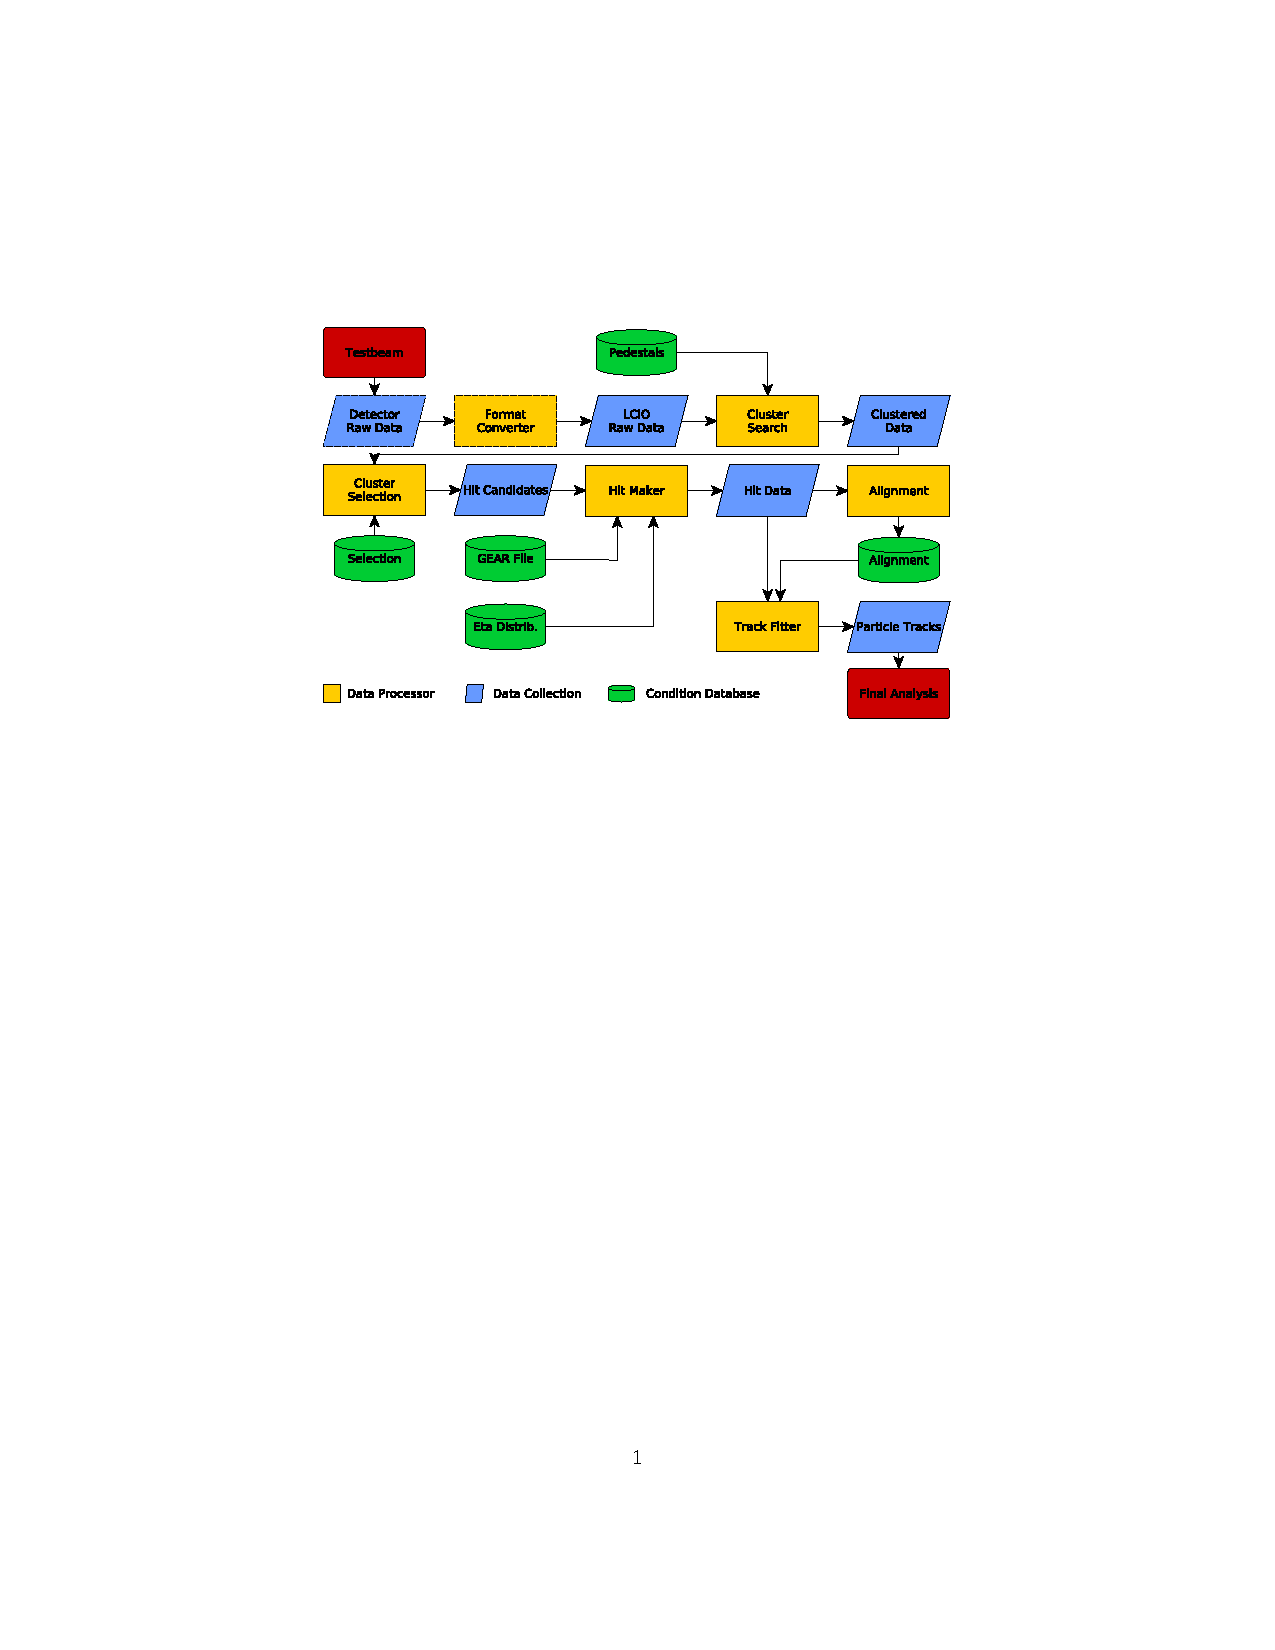
\includegraphics[width=\textwidth, trim = 30mm 150mm 30mm
      50mm, clip]{figures/Telescope/EUTelescope_pipeline.pdf}};
    \begin{scope}[x={(image.south east)},y={(image.north west)}]
    \end{scope}
  \end{tikzpicture} 
  \caption{Data reconstruction and analysis workflow using the
    EUTelescope framework. From~\cite{Jansen:2016bkd}.}
  \label{fig:EUTelescope_EUDET_pipeline}
\end{figure}

The EUTelescope framework was adapted for the reconstruction of the
data from the Timepix3 telescope. The framework is originally written
for a frame-based readout mode and had to be adapted to the
data-driven readout mode which was used during the data taking. This
affects mainly the definition of an event. In the frame-based mode, an
event corresponds to a time frame where the shutter of the detectors
are opened and all hits are integrated. When the shutter is closed,
there is a dead-time where no data is acquired and all the hits are
read out from the readout chips and recorded in a raw data
file. Whereas in the data-driven mode, the data are acquired as soon
as a pixel is hit (there is no shutter and almost no dead-time). The
hits are written in the raw file with their time-stamps coming from a
combination of the TOA and the FPGA timing from the SPIDR readout (see
\cref{sec:TimepixReadout}). They are not ordered in time in the raw
file since the readout chip does not send them in the order they are
produced. Pre-processing is needed to order the hits by their TOA and
create events as described below.

The reconstruction chain for the Timepix3 telescope is performed in
the following steps:

\begin{enumerate}
\item Converter: converts the raw files written by each telescope
  planes and the DUT in a binary format to an LCIO event. The
  converter also defines the event for the data-driven zero-suppressed
  readout mode and orders the hits.

  In the converter processor, the hits within a time window of 3~ms
  are read and filled into a vector. This time window is large enough
  to acquire all the hits belonging to many tracks. The hits in the
  vector are ordered in time according to their time-stamps. An LCIO
  event is built by choosing the hits in the six telescope planes and
  the DUT with time stamps differing by at most
  $2.5\,\microsecond$. With this constraint, in most cases one track
  per event is obtained (for particle rates of $\sim1$~million per
  second) and all hits belong to the same track. Only around half of
  the 3~ms time window is used to reconstruct the events. The other
  half is combined with the next 3~ms time window in order to avoid
  the loss of the hits in-between the time windows.

\item Hot pixels remover: hot pixels with the maximum allowed
  frequency of 0.1~Hz are discarded from the analysis. 
\item Clustering: the clusters in each telescope plane is found.
\item Hit making: reconstruction of the hit position for each cluster
  with the $\eta$-correction method~\cite{Belau:1983eh}.
\item Alignment: the alignment processor uses the Millepede~II
  algorithm~\cite{Blobel20065} to align the telescope planes with
  respect to each other. It assumes straight tracks and consists of a
  least squares minimisation method. A proper definition of the
  geometry is important for this step.
\item Track finding: the \texttt{EUTelTestFitter} algorithm
  implemented as a Marlin processor is used for finding and fitting
  the tracks. This track fitting method is based on a
  $\chi^2$-minimisation as described in~\cite{Zarnecki:2007yu}. Due to
  the multiple scatterings in the telescope planes, the tracks are
  displaced in the order of a few micrometers, which can not be
  neglected since it is comparable with the expected resolution of the
  telescope layers. This method is separately considered for the
  horizontal (x) and vertical (y) planes. The goal is to determine the
  position of the tracks on each telescope plane and the DUT from the
  measured positions on the telescope planes. The $\chi^2$ of the fit
  uses the additional constraint on the angles of the multiple
  scatterings. The track positions correspond to the positions
  minimising the $\chi^2$ distribution.

  The track positions on the DUT can be written in a ROOT
  tree~\cite{BRUN199781} and saved in a ROOT file. The raw data from
  the DUT is also written in the same file to be processed separately
  with the pyEudetAnalysis framework (see \cref{sec:pyEudetAnalysis}).
\end{enumerate} 

\subsection{pyEudetAnalysis}
\label{sec:pyEudetAnalysis}

Once the telescope tracks are reconstructed using the EUTelescope
framework, the analysis of the DUT can be done separately within the
python-based pyEudetAnalysis framework~\cite{pyeudet}. Separating the
telescope and the DUT analyses, provides more flexibility on the
analysis of the DUT. The tracks are reconstructed once and rerunning
of the analysis on the DUT does not require to reconstruct the tracks
one more time.

The pyEudetAnalysis reads the reconstructed track position and the
list of the pixels hit on the DUT from the ROOT file generated by
EUTelescope.
 
The workflow for pyEudetAnalysis is very similar to
EUTelescope. Except for the track reconstruction step which is not
needed in pyEudetAnalysis. The workflow is described
in~\cite{AlipourTehrani:2133128} and briefly summarised below:

\begin{enumerate}
\item Reading the output of the EUTelescope: the tracks and the pixels
  hit on the DUT are read from the ROOT file and stored in specified
  structures to be used for the analysis.

\item Hot pixel remover: noisy pixels on the DUT with a firing
  frequency higher than 0.01~Hz are removed from the analysis.

\item Clustering: the pixels hit on the DUT are clustered using the
  SciPy hierarchical \texttt{fclusterdata}
  algorithm~\cite{scipyClustering}.

\item Hit position reconstruction: pyEudetAnalysis provides several
  algorithms to reconstruct the position of the hits within the
  cluster. The $\eta$-correction method (see \cref{sec:EtaCorrection})
  is as well implemented which uses the TOT (charge) information to
  compensate for the non-linearities due to the charge sharing.

\item Track-hit alignment: the reconstructed tracks are compared to
  the reconstructed hit on the DUT. The hits are brought into lines
  with the tracks by defining translations in x and y directions
  during the pre-alignment procedure. The main alignment method
  consists of defining precisely the translation and rotations to
  precisely match the tracks to the matched hits. A metric defined as
  the radial distance between each track and the closest hit within a
  distance of less than 0.5mm. The Nelder-Mead method of SciPy
  \texttt{optimize.minimize}~\cite{SciPyOptimizeMinimize} is used to
  minimise the total distance. This function automatically varies the
  rotation about z and the x and y translations simultaneously to find
  the optimal alignment.

\item Track-hit matching: the alignment constants found previously are
  applied to the hits. The hits on the DUT are then matched to the
  tracks. This is done by taking the closest hit to each track, within
  a radial distance of 0.1~mm. The hits which are not connected to the
  tracks most probably belong to the electronics noise and are not
  related to the passing of particles and therefore discarded in the
  analysis. The DUT efficiency can be studied by using this track-hit
  matching.
\end{enumerate}
